\mychapter{Especificação do Projeto}
\label{Cap:especificacao}
\paragraph{
	O sistema será composto por duas partes: hardware, ou seja, os componentes como roteadores, processadores, sensores, entre outros; e software, identificado como o aplicativo de interface entre o usuário e os dados coletados.
}
\paragraph{
	O sistema está brevemente descrito através da Figura 1 e a disposição dos componentes através do diagrama de implantação da figura 2:
}
\begin{figure}
\centering
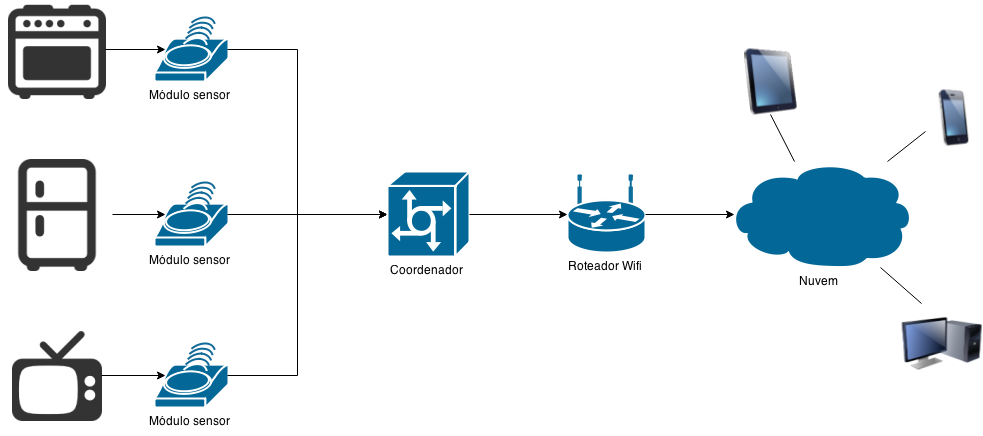
\includegraphics[width=1\textwidth]{figuras/esqueminha.png}
\caption{\label{fig:esqueminha} Esquema do Projeto}
\end{figure}

\begin{figure}
\centering
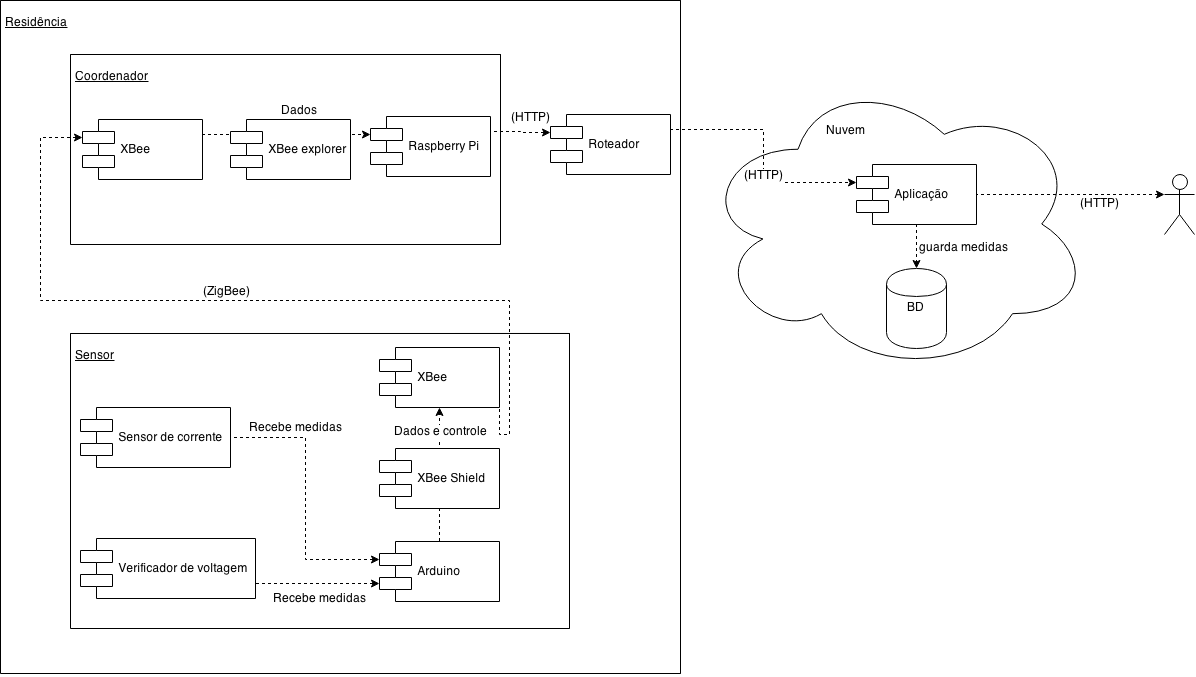
\includegraphics[width=1\textwidth]{figuras/diagrama_implantacao.png}
\caption{\label{fig:diagrama_implantacao} Diagrama de implantação}
\end{figure}
\paragraph{
	A parte de hardware está separado em dois módulos principais: o módulo de sensoriamento e um módulo coordenador e a parte de software se resume à parte da aplicação web na nuvem.
}
\section{Hardware}
\label{Sec:hardware}
\subsection{Módulo sensor}
\paragraph{
	O módulo sensor vai ser responsável por medir e transmitir as informações necessárias para calcular o consumo de energia do equipamento acoplado.
}
\paragraph{
	Os componentes físicos do módulo sensor são:
}
\begin{itemize}
\item Circuito Verificador de Voltagem
\item Sensor de Corrente (Non-invasive AC Current Sensor)
\item Arduino Uno - R3
\item XBee Shield
\item XBee 2mW PCB Antenna - Series 2
\end{itemize}

\subsection{Coordenador}
\paragraph{
	O módulo coordenador vai ser responsável por fazer requisições para os módulos sensores, tratar os dados de consumo e enviar ao aplicativo.
}
\paragraph{
	Os componentes do coordenador são:
}
\begin{itemize}
\item Kit Raspberry Pi2 + Fonte + Microsd 8gb + Wifi Usb
\item XBee Explorer Dongle
\item XBee 2mW PCB Antenna - Series 2
\end{itemize}

\subsection{Circuitos}
\subsubsection{Verificador de Tensão}
\paragraph{
No circuito de cada módulo de sensor, são feitas detecções da voltagem (110V ou 220V) para cálculos de potência. O circuito da Figura 3.3 foi simulado no PSpice para esse propósito, com componentes com parâmetros não finais, para uma análise lógica do bloco. O objetivo do circuito da figura dois é indicar se a tensão na tomada é 220V ou 110V, retornando 5V ou 0V, respectivamente.
}
\begin{figure}[H]
\centering
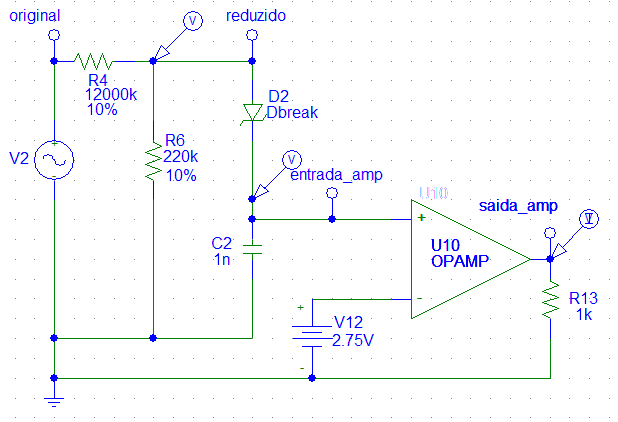
\includegraphics[width=1\textwidth]{figuras/voltage-circuit.png}
\caption{\label{fig:voltage-circuit} Diagrama de blocos do circuito que verifica a tensão}
\end{figure}

\subsection{Peças}
\subsubsection{Non-invasive AC current sensor}
\subsubsection{Raspberry Pi 2 modelo B}
\begin{figure}[H]
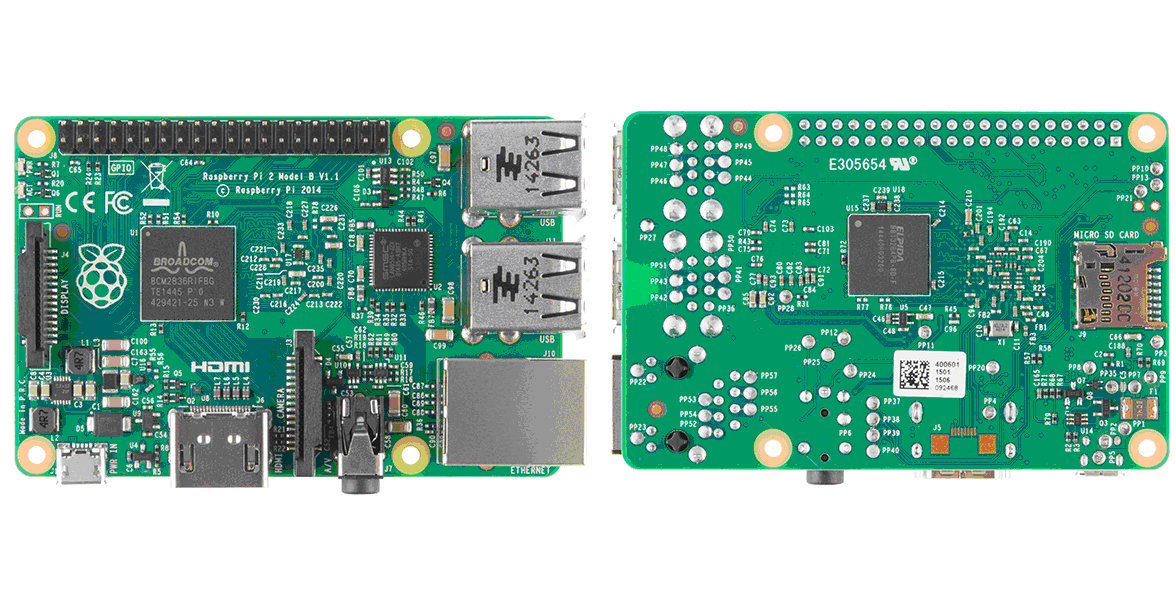
\includegraphics[width=1\textwidth]{figuras/raspberry_pi.png}
\caption{\label{fig:raspberry pi} Raspberry pi 2 modelo B}
\end{figure}
\paragraph{
A Raspberry Pi 2 Modelo B (figura 3.4) é o computador utilizado no sistema para receber os dados enviados pelos módulos sensores, tratá-los e enviar para o aplicativo. Foi escolhido o Raspberry Pi 2 - Model B por ser mais veloz, por possuir mais entradas USB e ser de alta disponibilidade no mercado, por um preço razoável. O kit inclui a fonte, um cartão microSD de 8GB e um adaptador Wifi USB.
}
\begin{itemize}
\item{A 900MHz quad-core ARM Cortex-A7 CPU}
\item{1GB RAM}
\item{40 pinos GPIO}
\item{saída Full HDMI}
\item{porta Ethernet}
\item{entrada para cartão Micro SD}
\item{4 entradas USB}
\end{itemize}

\subsubsection{Arduino UNO}
\begin{figure}[H]
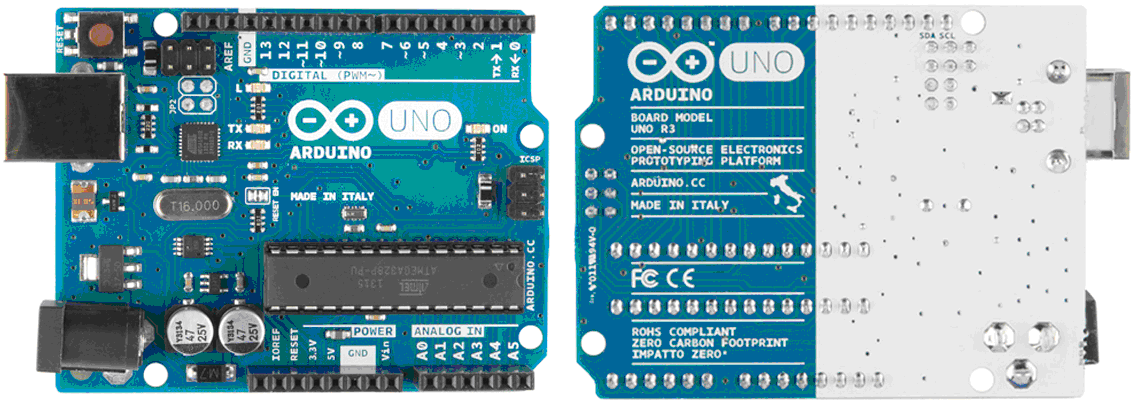
\includegraphics[width=1\textwidth]{figuras/arduino_uno.png}
\caption{\label{fig:arduino uno} Arduino UNO}
\end{figure}
\paragraph{
Arduino é uma placa programável open-source . No projeto em questão é utilizado como o microcontrolador, que receberá os dados do sensor, fará um tratamento e terá o envio programado desses para o coordenador. Pelo Arduino ser programável e possuir uma interface muito amigável, simplifica essa ponte entre a coleta de dados e a transmissão.
}
\begin{itemize}
\item{microcontrolador ATmega328}
\item{Voltagem de entrada - 7-12V}
\item{14 Pinos Digital I/O (6 PWM de saída)}
\item{6 Inputs Analógicos}
\item{32k de memória Flash}
\item{16Mhz de Relógio}
\end{itemize}

\subsubsection{XBee}
\begin{figure}[H]
\begin{center}
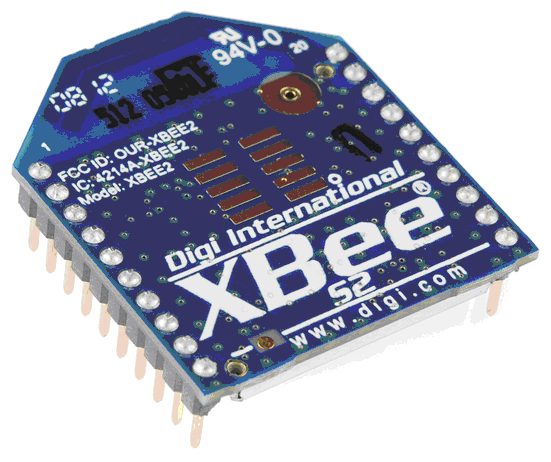
\includegraphics[width=5cm,height=5cm,keepaspectratio]{figuras/xbee_serie2.png}
\caption{\label{fig:xbee} XBee serie 2}
\end{center}
\end{figure}
\paragraph{
É um módulo que permite uma comunicação simples e confiável entre microcontroladores, computadores, sistemas através de uma porta serial. Pode ser utilizado em redes ponto-a-ponto e multi-ponto. Foram escolhidos módulos da série 2 pois são configuráveis.
Algumas outras especificações são:
}
\begin{itemize}
\item{entradas de 3.3V @ 40mA}
\item{transmissão de dados máxima de 250kbps}
\item{potência de saída: 2mW (+3dBm)}
\item{alcance mãximo de 120m}
\item{08 pinos digitais entrada/saída}
\item{encriptação 128-bit}
\item{configuração local ou remota}
\item{conector de antena RPSMA}
\end{itemize}

\subsubsection{XBee Explorer Dongle}
\begin{figure}[H]
\begin{center}
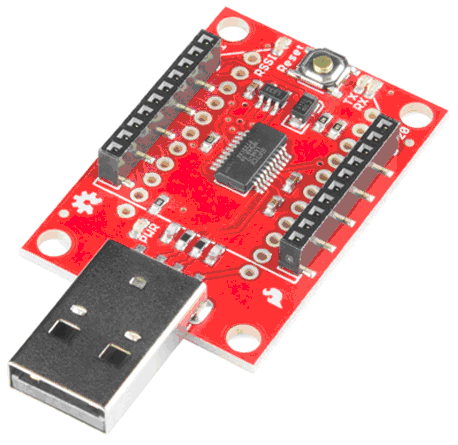
\includegraphics[width=5cm,height=5cm,keepaspectratio]{figuras/xbee_explorer_dongle.png}
\caption{\label{fig:xbee explorer dongle} XBee Explorer Dongle}
\end{center}
\end{figure}
\paragraph{
É um módulo com porta USB que faz a conexão do módulo XBee a um computador. Isso é necessário para ter acesso aos pinos de comunicação serial e de programação. Ele possui um conversor USB-serial, que traduz os dados entre o computador e o XBee. Possui um botão de reset e um regulador de voltagem para suprir a voltagem necessária para XBee. Além disso possui 4 leds para debug: RX, TX, RSSI e indicador de energia. No projeto, este módulo é utilizado para fazer as configurações iniciais de todos os XBees e para conectar o XBee coordenador ao Raspberry Pi.
}

\subsubsection{XBee Shield}
\begin{figure}[H]
\begin{center}
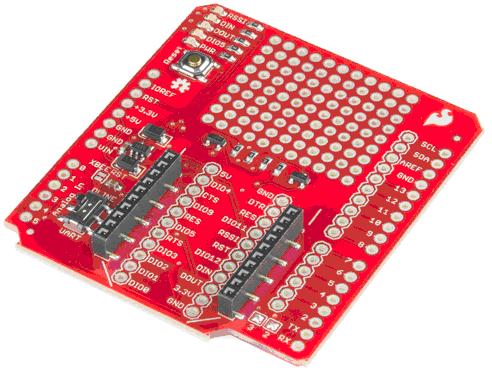
\includegraphics[width=5cm,height=5cm,keepaspectratio]{figuras/xbee_shield.png}
\caption{\label{fig:xbee shield} XBee shield do arduino UNO}
\end{center}
\end{figure}
\paragraph{
É um módulo que faz a conexão entre um módulo XBee e um Arduino. Ele possui opções para escolher se a conexão vai ser nos pinos UART ou qualquer outros pinos digitais do Arduino. A alimentação de 5V vinda do Arduino é regulada para 3.3V VDC antes de chegar no módulo XBee. O XBee Shield inclui LEDs para indicar a utilização dos pinos DIN, DOUT, RSSI e DIO5 do XBee. É usado um módulo XBee Shield para cada par XBee + Arduino.
}

\subsubsection{Arduino Stackable Header Kit - R3}
\begin{figure}[H]
\begin{center}
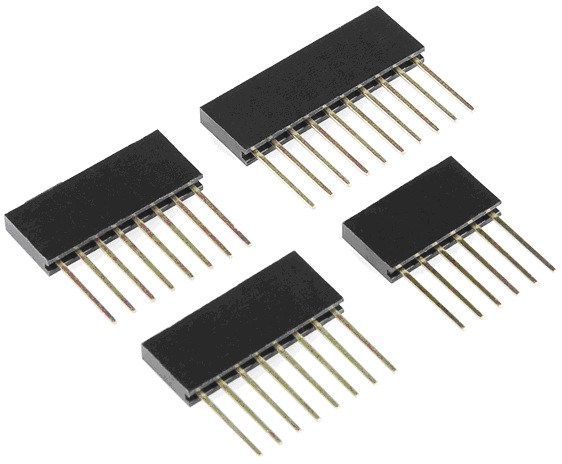
\includegraphics[width=5cm,height=5cm,keepaspectratio]{figuras/headers.png}
\caption{\label{fig:xbee shield headers} Headers usados no XBee shield}
\end{center}
\end{figure}
\paragraph{
São conectores usados para encaixar o módulo XBee Shield no Arduino Uno R3. Estão inclusos 4 headers, 2 x 8 pinos, 1 x 10 pinos e 1 x 6 pinos, suficientes para 1 módulo XBee Shield. Como há 2 sensores no projeto, serão usados 2 kits, com um adicional de reserva.
}

\section{Software}
\label{Sec:software}
\paragraph{
Coletado os dados, resta mostrar informações úteis ao usuário. Com o consumo de corrente e a voltagem da tomada, é possível calcular a potência e alguns outros dados interessantes para o usuário. O aplicativo desenvolvido nesse trabalho será responsável por esse tratamento e a visualização dos dados coletados pelos sensores. As funções principais são as seguintes:
}
\begin{itemize}
\item{realizar login}
\item{criar planos de consumo mensal máximo}
\item{visualizar o consumo através de gráficos por equipamento ou total}
\item{calcular o custo do consumo dos equipamentos por período}
\item{exportar os dados de consumo de um equipamento (ou mais)}
\item{importar os dados de consumo de um equipamento (ou mais)}
\end{itemize}
\subsection{Classes e atributos}
\textbf{Classe}: Equipment\\
\textbf{Descrição}: um equipamento monitorado\\	
\textbf{Atributos:}
\begin{enumerate}
  \item id (integer): Identificador do equipamento
  \item name (String): Nome do equipamento
  \item description (Text): descrição do equipamento 
  \item nominal\_power (float): potência do equipamento descrita no manual do equipamento 
  \item measurement\_unit (String): unidade do valor dado em nominal\_power
  \item approximated\_consumption (float): consumo aproximado do equipamento dado pelo fabricante 
\end{enumerate}

\textbf{Classe}: Sensor\\
\textbf{Descrição}: um sensor do sistema\\	
\textbf{Atributos:}
\begin{enumerate}
	\item id (integer): identificador do sensor dentro do software.
	\item name (String): nome dado pelo usuário para o sensor
	\item code (String): identificador do sensor entre outros sensores. Informação configurada no próprio módulo do sensor.
	\item equipment\_id (integer): equipamento a qual está associado
\end{enumerate}

\textbf{Classe}: Consumption\\
\textbf{Descrição}: Representa uma medida feita de um equipamento em um dado instante\\	
\textbf{Atributos:}
\begin{enumerate}
	\item id (integer): identificador do consumo
	\item moment (DateTime): a data e a hora de quando foi feita a medida
	\item current (float): corrente no momento da medida em amperes
	\item voltage (float): voltagem do tomada do equipamento. 220V ou 110V
\end{enumerate}

\subsection{Classes e atributos}
	\textbf{Classe}: User\\
	\textbf{Descrição}: Representa um usuário do sistema\\	
	\textbf{Atributos:}
\begin{enumerate}
	\item id (integer): identificador do usuário
	\item name (String):  Nome do usuário
	\item username (String): Nome de usuário usado para efetuar o login
	\item password (String com Criptografia): Senha do usuário usada para efetuar o login
    \item income\_type (String): O tipo de renda do usuário, Residencial ou Residencial de baixa renda, definida pela AES eletropaulo.
\end{enumerate}

\subsection{Classes e atributos}
	\textbf{Classe}: Goal\\
	\textbf{Descrição}: Representa uma meta de consumo por mês.\\
	\textbf{Atributos:}
\begin{enumerate}
	\item id (integer): identificador da meta
	\item name (String):  Nome da meta
	\item value\_in\_percent (float): Consumo pretendido em percentagem (em relação ao mês anterior)
	\item yearmonth\_start (DateTime): Mês/Ano de início do período da meta
    \item yearmonth\_end (DateTime): Mês/Ano de fim do período da meta
\end{enumerate}

\subsection{Classes e atributos}
	\textbf{Classe}: AESRate\\
	\textbf{Descrição}: Representa a taxa de conversão da AES eletropaulo de kilowatts hora para reais. Esses valores são obtidos através do site da AES Eletropaulo: \url{https://www.aeseletropaulo.com.br/poder-publico/prazos-e-tarifas/conteudo/tarifa-de-energia-eletrica}\\
	\textbf{Atributos:}
\begin{enumerate}
	\item id (integer): identificador da taxa de conversão
	\item value (float): O valor da taxa de conversão no instante
	\item date (DateTime): O instante que a taxa de conversão foi buscada
	\item range\_start (float): O início da faixa que define a taxa de conversão
    \item range\_end (float): O início da faixa que define a taxa de conversão
\end{enumerate}

\paragraph{No sistema é possível cadastrar apenas uma entidade principai os equipamentos eletrônicos monitorados, sendo prevista a possibilidade de que um sensor possa mudar de um equipamento para outro, sendo que tal mudança deve ser cadastrada no sistema pelo  usuário na tela de configurações, como mostrado na tela de configurações no diagrama de navegação.  Essa possibilidade de mudança da configuração dos sensores explica a relação do equipamento e as medidas de consumo: caso o usuário troque o sensor de equipamento ainda será possível visualizar dados anteriores de outros equipamentos já monitorados.
Os sensores devem ser criados automaticamente pelo sistema uma vez que eles sejam colocados no sistema. Eles enviam um sinal inicial que informa seu identificador para que o sistema o cadastre. O usuário poderá, então, colocar um nome que preferir nesse sensor.\\
Adquiridas as medidas, é possível vizualizar esses dados em uma tabela de consumo na tela de consumo. Nessa tela, é possível construir o gráfico do consumo em função de vários períodos de tempo, no caso, o consumo por dia e por mês, assim como metas de consumo de energia dos equipamentos selecionados e previsões de consumo que serão calculadas a partir do consumo nominal dos equipamentos.
}

\begin{figure}[H]
\begin{center}
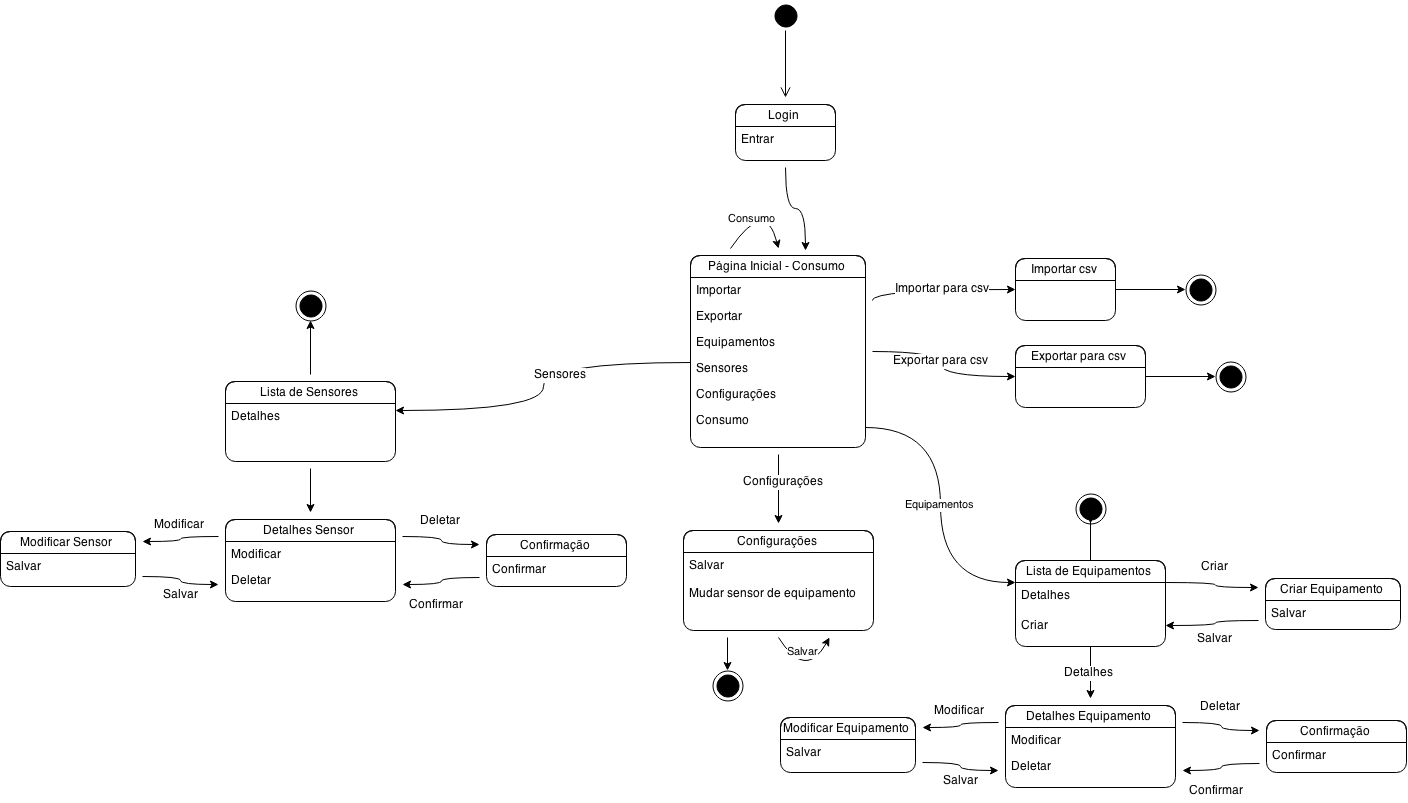
\includegraphics[width=10cm,height=10cm,keepaspectratio]{figuras/diagrama_navegacao.png}
\caption{\label{fig:diagrama navegacao} Diagrama de Navegação}
\end{center}
\end{figure}

\begin{figure}[H]
\begin{center}
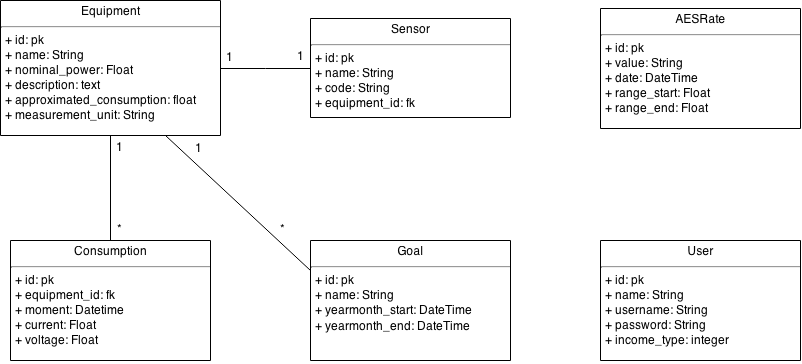
\includegraphics[width=10cm,height=10cm,keepaspectratio]{figuras/diagrama_classes.png}
\caption{\label{fig:diagrama classes} Diagrama de Classes}
\end{center}
\end{figure}

\subsection{Regras de negócio}
\paragraph{As medidas serão feitos em uma taxa de uma vez a cada dez minutos, o que leva a 6 amostras por hora, 144 por dia e 4320 por mês. Dado que cada amostra é uma linha de uma tabela, torna-se necessário algum tipo de redução desses dados para que o banco na nuvem não chegue a seu ponto máximo, dado que no projeto será usado um serviço cloud com taxa gratuita e, portanto, muito limitada. Logo, foi decidido que a janela temporal que o usuário conseguirá visualizar será restrita ao mês anterior e o mês atual quando o gráfico for uma função das horas do dia, e os outros dados mais antigos serão agrupados em meses para que ainda possa ser possível visualiza-los quando o gráfico for uma função dos meses. Caso seja necessário, será usado um plano pago, o que resolveria esse problema.
}

\subsection{Tecnologia}
\paragraph{Para o aplicativo será utilizado o framework Django, devido ao uso da linguagem python, que é uma linguagem limpa, de fácil utilização e com ampla disponibilidade de bibliotecas gratuitas e de fóruns para auxílio na implementação.
}